% Options for packages loaded elsewhere
\PassOptionsToPackage{unicode}{hyperref}
\PassOptionsToPackage{hyphens}{url}
\documentclass[
  11pt,
]{article}
\usepackage{xcolor}
\usepackage[left=3cm,right=3cm,top=2.5cm,bottom=2.5cm]{geometry}
\usepackage{amsmath,amssymb}
\setcounter{secnumdepth}{-\maxdimen} % remove section numbering
\usepackage{iftex}
\ifPDFTeX
  \usepackage[T1]{fontenc}
  \usepackage[utf8]{inputenc}
  \usepackage{textcomp} % provide euro and other symbols
\else % if luatex or xetex
  \usepackage{unicode-math} % this also loads fontspec
  \defaultfontfeatures{Scale=MatchLowercase}
  \defaultfontfeatures[\rmfamily]{Ligatures=TeX,Scale=1}
\fi
\usepackage{lmodern}
\ifPDFTeX\else
  % xetex/luatex font selection
\fi
% Use upquote if available, for straight quotes in verbatim environments
\IfFileExists{upquote.sty}{\usepackage{upquote}}{}
\IfFileExists{microtype.sty}{% use microtype if available
  \usepackage[]{microtype}
  \UseMicrotypeSet[protrusion]{basicmath} % disable protrusion for tt fonts
}{}
\usepackage{setspace}
\makeatletter
\@ifundefined{KOMAClassName}{% if non-KOMA class
  \IfFileExists{parskip.sty}{%
    \usepackage{parskip}
  }{% else
    \setlength{\parindent}{0pt}
    \setlength{\parskip}{6pt plus 2pt minus 1pt}}
}{% if KOMA class
  \KOMAoptions{parskip=half}}
\makeatother
\usepackage{longtable,booktabs,array}
\usepackage{caption}
\captionsetup[table]{skip=6pt}
\newcounter{none} % for unnumbered tables
\usepackage{calc} % for calculating minipage widths
% Correct order of tables after \paragraph or \subparagraph
\usepackage{etoolbox}
\makeatletter
\patchcmd\longtable{\par}{\if@noskipsec\mbox{}\fi\par}{}{}
\makeatother
% Allow footnotes in longtable head/foot
\IfFileExists{footnotehyper.sty}{\usepackage{footnotehyper}}{\usepackage{footnote}}
\makesavenoteenv{longtable}
\usepackage{graphicx}
\makeatletter
\newsavebox\pandoc@box
\newcommand*\pandocbounded[1]{% scales image to fit in text height/width
  \sbox\pandoc@box{#1}%
  \Gscale@div\@tempa{\textheight}{\dimexpr\ht\pandoc@box+\dp\pandoc@box\relax}%
  \Gscale@div\@tempb{\linewidth}{\wd\pandoc@box}%
  \ifdim\@tempb\p@<\@tempa\p@\let\@tempa\@tempb\fi% select the smaller of both
  \ifdim\@tempa\p@<\p@\scalebox{\@tempa}{\usebox\pandoc@box}%
  \else\usebox{\pandoc@box}%
  \fi%
}
% Set default figure placement to htbp
\def\fps@figure{htbp}
\makeatother
\setlength{\emergencystretch}{3em} % prevent overfull lines
\providecommand{\tightlist}{%
  \setlength{\itemsep}{0pt}\setlength{\parskip}{0pt}}
% Statistics in Medicine submission preamble.
% Shared across analysis/report/<paper>/report.Rmd files via
%   includes:
%     in_header: ../sim-preamble.tex
% in the YAML output block.
%
% The page footer (source path, render time, version) is no
% longer set here. It is supplied at render time by the vendored
% tools/stamp-render.R, which injects tools/stamp.tex.

% Continuous line numbering for editorial review. The 'mathlines'
% option extends numbering through display-math environments
% (equation, align, ...), which SIM editorial workflows expect.
\usepackage[mathlines]{lineno}
\linenumbers
\usepackage{amsmath}

% Spacing: linestretch is set in YAML (1.5 line spacing).
\usepackage{setspace}
%% tools/stamp.tex
%% Provenance footer for PDFs rendered from this project.
%% Vendored by zzcollab; this file is not project-specific. The
%% footer prints the source document and the time of rendering.
%% The git version is defined here too, and so is available to a
%% project that wants it on the page, but it is left off the
%% default footer: it already names the staged copy in share/ and
%% appears in its manifest row. All values are supplied at render
%% time by tools/stamp-render.R, which writes a small generated
%% file that redefines the macros below. The \providecommand
%% defaults keep a bare LaTeX compile working when the document is
%% built without the wrapper.
\usepackage{fancyhdr}
\usepackage{xcolor}
\providecommand{\stampsource}{\detokenize{(source not recorded)}}
\providecommand{\stamptime}{(time not recorded)}
\providecommand{\stampversion}{\detokenize{(version not recorded)}}
\setlength{\footskip}{40pt}
\newcommand{\stampfootcontent}{%
  \footnotesize\color{gray}%
  \parbox[b]{\textwidth}{%
    \stamptime\hfill\thepage\\[2pt]%
    \ttfamily\raggedright\stampsource}}
\pagestyle{fancy}
\fancyhf{}
\fancyfoot[C]{\stampfootcontent}
\renewcommand{\headrulewidth}{0pt}
\renewcommand{\footrulewidth}{0.4pt}
%% The title page uses the `plain` page style; redefine it so the
%% stamp appears there too.
\fancypagestyle{plain}{%
  \fancyhf{}%
  \fancyfoot[C]{\stampfootcontent}%
  \renewcommand{\headrulewidth}{0pt}%
  \renewcommand{\footrulewidth}{0.4pt}}
\renewcommand{\stampsource}{\textasciitilde{}/\allowbreak{}prj/\allowbreak{}res/\allowbreak{}36-pmsimstats-ng/\allowbreak{}pmsimstats-ng/\allowbreak{}analysis/\allowbreak{}report/\allowbreak{}02-carryover-sensitivity/\allowbreak{}summary.Rmd}
\renewcommand{\stamptime}{2026-10-28 09:05 PDT}
\renewcommand{\stampversion}{\detokenize{whitepapers-pre-series-103-gc195cd42b-wip}}
\usepackage{amsmath}
\usepackage{amssymb}
\usepackage{booktabs}
\usepackage{longtable}
\usepackage{float}
\AtBeginDocument{\nolinenumbers}
\usepackage{booktabs}
\usepackage{longtable}
\usepackage{array}
\usepackage{multirow}
\usepackage{wrapfig}
\usepackage{float}
\usepackage{colortbl}
\usepackage{pdflscape}
\usepackage{tabu}
\usepackage{threeparttable}
\usepackage{threeparttablex}
\usepackage[normalem]{ulem}
\usepackage{makecell}
\usepackage{xcolor}
\usepackage{bookmark}
\IfFileExists{xurl.sty}{\usepackage{xurl}}{} % add URL line breaks if available
\urlstyle{same}
% fallback for those not using the hyperref driver hyperxmp:
\makeatletter
\@ifundefined{xmpquote}{\newcommand{\xmpquote}[1]{#1}}{}
\makeatother
\hypersetup{
  pdftitle={Summary of paper 02: carryover representation and inference for biomarker-treatment interaction tests in aggregated N-of-1 trials under the correlation encoding of the interaction},
  pdfauthor={pmsimstats team},
  hidelinks,
  pdfcreator={LaTeX via pandoc}}

\title{Summary of paper 02: carryover representation and inference for biomarker-treatment interaction tests in aggregated N-of-1 trials under the correlation encoding of the interaction}
\author{pmsimstats team}
\date{October 28, 2026}

\begin{document}
\maketitle

\setstretch{1.1}
\section*{Problem and approach}\label{problem-and-approach}
\addcontentsline{toc}{section}{Problem and approach}

Aggregated N-of-1 trials pool repeated within-patient on/off contrasts to validate predictive biomarkers. Drug carryover attenuates the biomarker-by-treatment interaction. The analyst must decide how to represent residual exposure, how to obtain a correctly sized test, and whether to guard against a prognostic biomarker. We ran an exploratory, staged simulation study under the extended DGP, in which the interaction is a correlation between the biomarker and the drug response. Stage 1 compares three representations of residual exposure over 162 configurations. Stage 2 selects the half-life by AIC. Stage 3 adds CR2 inference and measures the cost of selection. Stage 4 adds the original analysis and an expectancy-term family. Stage 5 adds prognostic correlations, dropout and random slopes. The study ends in analysis G9: the exposure-weighted predictor with an AIC-selected half-life, refitted by REML and tested with CR2.

\section*{Simulation design}\label{simulation-design}
\addcontentsline{toc}{section}{Simulation design}

\subsection*{Estimand and analysis specifications}\label{estimand-and-analysis-specifications}
\addcontentsline{toc}{subsection}{Estimand and analysis specifications}

Table \ref{tab:tab-spec-summary} defines the nine specifications, G1 to G9. G1 to G3 represent residual exposure, G4 selects the half-life, and G6 to G9 add CR2 inference.

\begin{table}
\centering
\caption{\label{tab:tab-spec-summary}The nine G-family analysis specifications. G1-G3 are
    the Stage 1 representations of residual exposure; G4 replaces
    the assumed half-life by a data-driven choice (Stage 2); G6-G9
    are CR2 cluster-robust variants of G1, G2, G4 and G3 (Stage 3).
    G5 collapses to one row per patient before fitting and has no
    CR2 variant. The external comparators E0 and the F-family are
    defined in Section \ref{sec-comparators}.}
\centering
\resizebox{\ifdim\width>\linewidth\linewidth\else\width\fi}{!}{
\fontsize{9}{11}\selectfont
\begin{tabular}[t]{lllll}
\toprule
Code & Stored & Name & Formula & Target coefficient\\
\midrule
G1 & E1 & Unadjusted & Sx ~ bm + t + Db + bm:Db & bm:Db\\
G2 & E3 & Lag-adjusted & Sx ~ bm + t + Db + bm:Db + L & bm:Db\\
G3 & E2 & Exposure-weighted & Sx ~ bm + t + Dbc + bm:Dbc & bm:Dbc\\
G4 & E7 & AIC-selected t1/2 & G3 formula, t1/2 by AIC over \{0.25,0.5,1.0,2.0\} & bm:Dbc\\
G5 & E9 & Paired-difference & diff ~ bm (patient-level OLS) & bm slope\\
\addlinespace
G6 & E1cr2 & Unadjusted + CR2 & G1 formula, CR2 SE & bm:Db\\
G7 & E3cr2 & Lag-adjusted + CR2 & G2 formula, CR2 SE & bm:Db\\
G8 & E2cr2 & Exposure-weighted + CR2 & G3 formula, CR2 SE & bm:Dbc\\
G9 & E7cr2 & AIC-selected t1/2 + CR2 & G4 formula, CR2 SE & bm:Dbc\\
\bottomrule
\end{tabular}}
\end{table}

\section*{Results}\label{results}
\addcontentsline{toc}{section}{Results}

\subsection*{Stage 1: representing residual exposure}\label{stage-1-representing-residual-exposure}
\addcontentsline{toc}{subsection}{Stage 1: representing residual exposure}

Table \ref{tab:headline} gives the reference cell: Hybrid design, \(N = 70\), biomarker-response correlation 0.45. At a half-life of 1 week, power is 0.806 for G1, 0.808 for G2 and 0.888 for G3.

\begin{table}
\centering
\caption{\label{tab:headline}Stage 1: performance at the reference cell
    (exponential DGP, Hybrid design, $N = 70$,
    $c_{bm} = 0.45$, $n_{sim} = 500$). Power is the rejection rate of
    $H_0: \beta_{bm:X} = 0$ at $\alpha = 0.05$. Bias is
    mean(estimate $-$ $\theta_{\text{true}}$) on the calibrated
    effect-size scale, $\theta_{\text{true}} = -c_{bm}
    \cdot \sigma_{BR} = -3.6$; see the estimand-mismatch caveat in
    the text for G1/G2. Empirical SE is the standard deviation of the
    point estimates across replicates. Coverage is the proportion of
    nominal 95\% Wald CIs containing $\theta_{\text{true}}$. MSE is
    bias$^2$ + Empirical SE$^2$. Non-conv is the fraction of
    replicates where `nlme::lme()` failed to converge. MCSEs follow
    Morris et al. (2019, Table 6).}
\centering
\resizebox{\ifdim\width>\linewidth\linewidth\else\width\fi}{!}{
\begin{tabular}[t]{rlllllll}
\toprule
t1/2 & Specification & Power (MCSE) & Bias (MCSE) & Empirical SE & Coverage (MCSE) & MSE (MCSE) & Non-conv\\
\midrule
0.0 & Unadjusted & 0.994 (0.003) & -0.021 (0.031) & 0.699 & 0.990 (0.004) & 0.489 (0.029) & 0.000\\
0.0 & Lag-adjusted & 0.994 (0.003) & -0.022 (0.031) & 0.698 & 0.990 (0.004) & 0.487 (0.029) & 0.000\\
0.0 & Exposure-weighted & 0.994 (0.003) & -0.021 (0.031) & 0.699 & 0.990 (0.004) & 0.489 (0.029) & 0.000\\
0.5 & Unadjusted & 0.946 (0.010) & +0.618 (0.034) & 0.760 & 0.938 (0.011) & 0.959 (0.055) & 0.000\\
0.5 & Lag-adjusted & 0.944 (0.010) & +0.619 (0.034) & 0.762 & 0.936 (0.011) & 0.964 (0.055) & 0.000\\
\addlinespace
0.5 & Exposure-weighted & 0.962 (0.009) & +0.069 (0.039) & 0.873 & 0.970 (0.008) & 0.766 (0.052) & 0.000\\
1.0 & Unadjusted & 0.806 (0.018) & +1.143 (0.036) & 0.799 & 0.790 (0.018) & 1.943 (0.092) & 0.000\\
1.0 & Lag-adjusted & 0.808 (0.018) & +1.143 (0.036) & 0.808 & 0.786 (0.018) & 1.959 (0.092) & 0.000\\
1.0 & Exposure-weighted & 0.888 (0.014) & -0.084 (0.047) & 1.062 & 0.964 (0.008) & 1.135 (0.074) & 0.000\\
\bottomrule
\end{tabular}}
\end{table}

Figure \ref{fig:fig-power-by-spec} shows power against the half-life. The G1 and G2 curves coincide, and G3 falls less as the half-life grows.

\begin{figure}
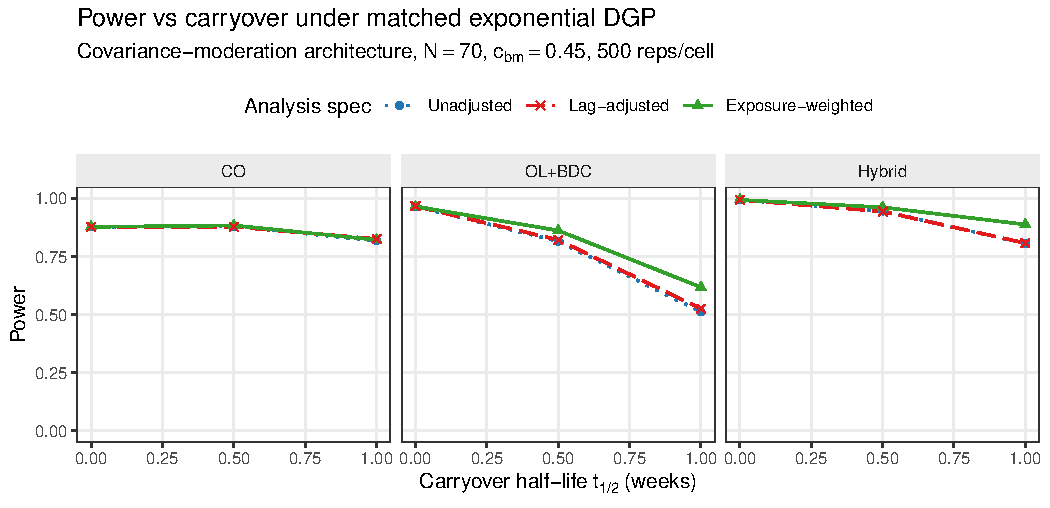
\includegraphics[width=0.95\linewidth]{../../figures/02xs-power-by-spec} \caption{Stage 1: power versus carryover half-life under the exponential DGP, by analysis specification and trial design ($c_{bm} = 0.45$, $n_{sim} = 500$).}\label{fig:fig-power-by-spec}
\end{figure}

\subsection*{Stage 2: removing the analyst's half-life}\label{stage-2-removing-the-analysts-half-life}
\addcontentsline{toc}{subsection}{Stage 2: removing the analyst's half-life}

Table \ref{tab:stage2} adds G4, which chooses the half-life from the data. For Hybrid, \(N = 70\), \(c_{bm} = 0.45\) and \(t_{1/2} = 1\), power is 0.790 for G1, 0.886 for G3 and 0.876 for G4.

\begin{table}
\centering
\caption{\label{tab:stage2}Stage 2: power of the binary indicator (G1), the
    exposure-weighted predictor at the true half-life (G3) and the
    exposure-weighted predictor at the AIC-selected half-life (G4),
    model-based inference, on the 30-cell corrected grid
    (exponential DGP, $n_{sim} = 500$, same simulated trial for all
    three each replicate). Two-MCSE half-width is about 0.04 at
    $p = 0.5$.}
\centering
\fontsize{9}{11}\selectfont
\begin{tabular}[t]{lrrrlll}
\toprule
Design & $N$ & $c_{bm}$ & $t_{1/2}$ & G1 & G3 & G4\\
\midrule
CO & 35 & 0.45 & 0.0 & 0.582 & 0.582 & 0.582\\
CO & 35 & 0.45 & 0.5 & 0.576 & 0.572 & 0.580\\
CO & 35 & 0.30 & 1.0 & 0.280 & 0.280 & 0.294\\
CO & 35 & 0.45 & 1.0 & 0.514 & 0.524 & 0.532\\
CO & 70 & 0.45 & 0.0 & 0.880 & 0.880 & 0.878\\
\addlinespace
CO & 70 & 0.45 & 0.5 & 0.874 & 0.874 & 0.874\\
CO & 70 & 0.30 & 1.0 & 0.508 & 0.518 & 0.522\\
CO & 70 & 0.45 & 1.0 & 0.832 & 0.852 & 0.844\\
Hybrid & 35 & 0.45 & 0.0 & 0.826 & 0.826 & 0.816\\
Hybrid & 35 & 0.45 & 0.5 & 0.656 & 0.678 & 0.688\\
\addlinespace
Hybrid & 35 & 0.30 & 1.0 & 0.212 & 0.250 & 0.276\\
Hybrid & 35 & 0.45 & 1.0 & 0.450 & 0.524 & 0.534\\
Hybrid & 70 & 0.45 & 0.0 & 0.992 & 0.992 & 0.990\\
Hybrid & 70 & 0.45 & 0.5 & 0.960 & 0.960 & 0.962\\
Hybrid & 70 & 0.30 & 1.0 & 0.448 & 0.518 & 0.534\\
\addlinespace
Hybrid & 70 & 0.45 & 1.0 & 0.790 & 0.886 & 0.876\\
OL+BDC & 35 & 0.45 & 0.0 & 0.694 & 0.694 & 0.700\\
OL+BDC & 35 & 0.45 & 0.5 & 0.474 & 0.506 & 0.523\\
OL+BDC & 35 & 0.30 & 1.0 & 0.134 & 0.164 & 0.182\\
OL+BDC & 35 & 0.45 & 1.0 & 0.248 & 0.330 & 0.344\\
\addlinespace
OL+BDC & 70 & 0.45 & 0.0 & 0.958 & 0.958 & 0.960\\
OL+BDC & 70 & 0.45 & 0.5 & 0.820 & 0.842 & 0.842\\
OL+BDC & 70 & 0.30 & 1.0 & 0.276 & 0.338 & 0.346\\
OL+BDC & 70 & 0.45 & 1.0 & 0.544 & 0.638 & 0.639\\
\bottomrule
\end{tabular}
\end{table}

\subsection*{Stage 3: a correctly sized test}\label{stage-3-a-correctly-sized-test}
\addcontentsline{toc}{subsection}{Stage 3: a correctly sized test}

Table \ref{tab:tab-type1-cr2} shows the model-based test rejecting at 0.033 to 0.046 under the null. CR2 moves the rejection rate to 0.046 to 0.059, and G4 is highest.

\begin{table}
\centering
\caption{\label{tab:tab-type1-cr2}Stage 3: conservatism of the model-based interaction
    test and its cluster-robust correction at four Hybrid null cells
    ($c_{bm} = 0$, exponential DGP, corrected simulation code,
    2{,}000 replicates each). $\kappa$ is the calibration ratio of
    Section 2.4; $\kappa > 1$ is a conservative test. The CR2
    columns are G6, G8 and G9 for G1, G3 and G4 respectively.
    Two-MCSE band around 0.05: $[0.040, 0.060]$.}
\centering
\fontsize{9}{11}\selectfont
\begin{tabular}[t]{lrlllll}
\toprule
$t_{1/2}$ & $N$ & Specification & $\kappa$ model & Type I model & $\kappa$ CR2 & Type I CR2\\
\midrule
0.5 & 35 & G1 & 1.05 & 0.041 & 0.97 & 0.049\\
0.5 & 35 & G3 & 1.05 & 0.035 & 0.97 & 0.050\\
0.5 & 35 & G4 & 1.00 & 0.043 & 0.93 & 0.056\\
0.5 & 70 & G1 & 1.05 & 0.042 & 0.98 & 0.050\\
0.5 & 70 & G3 & 1.06 & 0.037 & 0.99 & 0.050\\
\addlinespace
0.5 & 70 & G4 & 1.05 & 0.040 & 0.98 & 0.052\\
1.0 & 35 & G1 & 1.05 & 0.040 & 0.97 & 0.047\\
1.0 & 35 & G3 & 1.06 & 0.033 & 0.98 & 0.052\\
1.0 & 35 & G4 & 0.99 & 0.046 & 0.91 & 0.059\\
1.0 & 70 & G1 & 1.05 & 0.041 & 0.98 & 0.049\\
\addlinespace
1.0 & 70 & G3 & 1.07 & 0.035 & 0.99 & 0.046\\
1.0 & 70 & G4 & 1.03 & 0.042 & 0.96 & 0.055\\
\bottomrule
\end{tabular}
\end{table}

Table \ref{tab:stage3-pooled} pools the four null cells. G9 rejects at 0.0555 against 0.0493 for G8, a paired difference of 0.0059 (MCSE 0.0013).

\begin{table}
\centering
\caption{\label{tab:stage3-pooled}Stage 3: null rejection of G6, G8 and G9 pooled over
      the four 2{,}000-replicate Hybrid null cells of Table
      \ref{tab:tab-type1-cr2}; the paired difference between G9
      and G8 on the same trials (the discordant counts are 77
      replicates rejected by G9 only and 30 by G8 only); and G9
      conditional on the half-life it selected. From
      `34-referee-reanalysis.R`.}
\centering
\fontsize{9}{11}\selectfont
\begin{tabular}[t]{llrll}
\toprule
Quantity & Method & $n$ & Rate & MCSE\\
\midrule
Pooled null rejection & G6 & 7986 & 0.0486 & 0.0024\\
Pooled null rejection & G8 & 7988 & 0.0493 & 0.0024\\
Pooled null rejection & G9 & 7987 & 0.0555 & 0.0026\\
Paired difference, G9 minus G8 & G9-G8 & 7980 & 0.0059 & 0.0013\\
G9 given selected $\hat t^{a}_{1/2}$ = 0.25 & G9 & 3116 & 0.0507 & 0.0039\\
G9 given selected $\hat t^{a}_{1/2}$ = 0.5 & G9 & 2232 & 0.0587 & 0.0050\\
G9 given selected $\hat t^{a}_{1/2}$ = 1 & G9 & 1613 & 0.0583 & 0.0058\\
G9 given selected $\hat t^{a}_{1/2}$ = 2 & G9 & 1026 & 0.0585 & 0.0073\\
\bottomrule
\end{tabular}
\end{table}

Table \ref{tab:stage3-selection} shows that AIC selection does not recover the half-life. At a true half-life of 0.5 week and \(N = 70\), the smallest candidate is chosen in 0.59 of replicates and 0.5 week in 0.33.

\begin{table}
\centering
\caption{\label{tab:stage3-selection}Stage 3: share of replicates in which each candidate
      half-life (weeks) was selected by AIC, Hybrid design, pooled
      over every stored cell at the given true half-life and $N$
      (null and alternative cells together). From
      `34-referee-reanalysis.R`.}
\centering
\fontsize{9}{11}\selectfont
\begin{tabular}[t]{rrrllll}
\toprule
\multicolumn{3}{c}{ } & \multicolumn{4}{c}{Selected half-life} \\
\cmidrule(l{3pt}r{3pt}){4-7}
True $t_{1/2}$ & $N$ & $n$ & 0.25 & 0.5 & 1 & 2\\
\midrule
0.0 & 35 & 500 & 0.97 & 0.02 & 0.00 & 0.00\\
0.0 & 70 & 500 & 0.99 & 0.01 & 0.00 & 0.00\\
0.2 & 35 & 1000 & 0.95 & 0.05 & 0.00 & 0.00\\
0.2 & 70 & 992 & 0.98 & 0.02 & 0.00 & 0.00\\
0.5 & 35 & 34957 & 0.56 & 0.29 & 0.11 & 0.04\\
0.5 & 70 & 47337 & 0.59 & 0.33 & 0.06 & 0.01\\
1.0 & 35 & 3500 & 0.20 & 0.24 & 0.29 & 0.28\\
1.0 & 70 & 3493 & 0.12 & 0.26 & 0.40 & 0.21\\
2.0 & 35 & 1000 & 0.16 & 0.07 & 0.14 & 0.63\\
2.0 & 70 & 1992 & 0.06 & 0.06 & 0.15 & 0.73\\
4.0 & 35 & 1000 & 0.26 & 0.06 & 0.07 & 0.60\\
4.0 & 70 & 991 & 0.18 & 0.03 & 0.07 & 0.72\\
\bottomrule
\end{tabular}
\end{table}

\subsubsection*{Selection on the null model and fixed half-lives}\label{selection-on-the-null-model-and-fixed-half-lives}
\addcontentsline{toc}{subsubsection}{Selection on the null model and fixed half-lives}

Table \ref{tab:stage3-variants-null} compares selection variants. At \(t_{1/2} = 1.0\), \(N = 35\) and \(c_{PB} = 0\), G9 rejects at 0.0596, G9-null at 0.0506 and G8 at 0.0508.

\begin{table}
\centering
\caption{\label{tab:stage3-variants-null}Stage 3, referee-variant runs: null rejection rate
      ($c_{bm} = 0$) of G8, G9, G9-null, G8 at two fixed analysis
      half-lives and F1 in eight Hybrid null cells, 5{,}000
      replicates each (MCSE about 0.003), independent seeds per cell,
      with the paired per-replicate difference against G8 (paired SE
      0.0015 to 0.0021) and the calibration ratio. $c_{PB}$: a
      prognostic correlation with the placebo-response component.}
\centering
\fontsize{8}{10}\selectfont
\begin{tabular}[t]{lllll}
\toprule
Cell & Method & Rejection & Paired diff. vs G8 & $\kappa$\\
\midrule
$t_{1/2} = 0.5$, $N = 35$, $c_{PB} = 0.0$ & G8 & 0.0482 & -- & 0.97\\
 & G9 & 0.0522 & +0.0040 & 0.93\\
 & G9-null & 0.0470 & -0.0012 & 0.97\\
 & G8 at 0.25 wk & 0.0460 & -0.0022 & 0.98\\
 & G8 at 1.00 wk & 0.0462 & -0.0020 & 0.96\\
 & F1 & 0.0466 & -0.0016 & 0.98\\
$t_{1/2} = 0.5$, $N = 35$, $c_{PB} = 0.3$ & G8 & 0.0524 & -- & 0.96\\
 & G9 & 0.0584 & +0.0060 & 0.91\\
 & G9-null & 0.0532 & +0.0008 & 0.95\\
 & G8 at 0.25 wk & 0.0544 & +0.0020 & 0.96\\
 & G8 at 1.00 wk & 0.0510 & -0.0014 & 0.96\\
 & F1 & 0.0526 & +0.0002 & 0.96\\
$t_{1/2} = 0.5$, $N = 70$, $c_{PB} = 0.0$ & G8 & 0.0514 & -- & 0.99\\
 & G9 & 0.0538 & +0.0024 & 0.97\\
 & G9-null & 0.0510 & -0.0004 & 0.98\\
 & G8 at 0.25 wk & 0.0521 & +0.0008 & 0.98\\
 & G8 at 1.00 wk & 0.0492 & -0.0022 & 0.99\\
 & F1 & 0.0487 & -0.0026 & 0.99\\
$t_{1/2} = 0.5$, $N = 70$, $c_{PB} = 0.3$ & G8 & 0.0503 & -- & 0.99\\
 & G9 & 0.0544 & +0.0038 & 0.98\\
 & G9-null & 0.0508 & +0.0002 & 1.00\\
 & G8 at 0.25 wk & 0.0494 & -0.0010 & 0.99\\
 & G8 at 1.00 wk & 0.0508 & +0.0002 & 0.99\\
 & F1 & 0.0492 & -0.0016 & 0.99\\
$t_{1/2} = 1.0$, $N = 35$, $c_{PB} = 0.0$ & G8 & 0.0508 & -- & 0.96\\
 & G9 & 0.0596 & +0.0088 & 0.89\\
 & G9-null & 0.0506 & -0.0002 & 0.94\\
 & G8 at 0.25 wk & 0.0504 & -0.0004 & 0.96\\
 & G8 at 1.00 wk & 0.0508 & +0.0000 & 0.96\\
 & F1 & 0.0512 & +0.0004 & 0.97\\
$t_{1/2} = 1.0$, $N = 35$, $c_{PB} = 0.3$ & G8 & 0.0432 & -- & 0.98\\
 & G9 & 0.0536 & +0.0104 & 0.91\\
 & G9-null & 0.0422 & -0.0010 & 0.96\\
 & G8 at 0.25 wk & 0.0416 & -0.0016 & 0.99\\
 & G8 at 1.00 wk & 0.0432 & +0.0000 & 0.98\\
 & F1 & 0.0380 & -0.0052 & 0.99\\
$t_{1/2} = 1.0$, $N = 70$, $c_{PB} = 0.0$ & G8 & 0.0461 & -- & 1.00\\
 & G9 & 0.0505 & +0.0044 & 0.95\\
 & G9-null & 0.0447 & -0.0012 & 0.99\\
 & G8 at 0.25 wk & 0.0427 & -0.0036 & 1.00\\
 & G8 at 1.00 wk & 0.0461 & +0.0000 & 1.00\\
 & F1 & 0.0428 & -0.0034 & 1.00\\
$t_{1/2} = 1.0$, $N = 70$, $c_{PB} = 0.3$ & G8 & 0.0554 & -- & 0.95\\
 & G9 & 0.0634 & +0.0080 & 0.90\\
 & G9-null & 0.0568 & +0.0012 & 0.94\\
 & G8 at 0.25 wk & 0.0567 & +0.0010 & 0.95\\
 & G8 at 1.00 wk & 0.0554 & +0.0000 & 0.95\\
 & F1 & 0.0546 & -0.0010 & 0.95\\
\bottomrule
\end{tabular}
\end{table}

Table \ref{tab:stage3-variants-alt} gives power. At a true half-life of 2 weeks and \(N = 70\) with \(c_{bm} = 0.45\), power is 0.679 for G8, 0.515 for G9, 0.667 for G9-null and 0.661 for G8 fixed at 1 week.

\begin{table}
\centering
\caption{\label{tab:stage3-variants-alt}Stage 3, referee-variant runs: power at eight Hybrid
      alternative cells, 1{,}000 replicates each (MCSE at most 0.016),
      independent seeds per cell, for the same analyses as the null
      table. The true half-life is 0.5 or 2 weeks; the fixed analysis
      half-lives are 0.25 and 1 week in every cell.}
\centering
\fontsize{9}{11}\selectfont
\begin{tabular}[t]{rrrllllll}
\toprule
$t_{1/2}$ & $N$ & $c_{bm}$ & G8 & G9 & G9-null & G8 at 0.25 wk & G8 at 1 wk & F1\\
\midrule
0.5 & 35 & 0.25 & 0.291 & 0.293 & 0.277 & 0.276 & 0.273 & 0.267\\
0.5 & 70 & 0.25 & 0.538 & 0.538 & 0.526 & 0.517 & 0.517 & 0.514\\
0.5 & 35 & 0.45 & 0.743 & 0.753 & 0.737 & 0.735 & 0.723 & 0.715\\
0.5 & 70 & 0.45 & 0.966 & 0.964 & 0.960 & 0.958 & 0.959 & 0.951\\
2.0 & 35 & 0.25 & 0.124 & 0.139 & 0.108 & 0.097 & 0.117 & 0.088\\
2.0 & 70 & 0.25 & 0.248 & 0.271 & 0.239 & 0.187 & 0.256 & 0.180\\
2.0 & 35 & 0.45 & 0.384 & 0.410 & 0.362 & 0.307 & 0.370 & 0.288\\
2.0 & 70 & 0.45 & 0.679 & 0.690 & 0.661 & 0.515 & 0.667 & 0.483\\
\bottomrule
\end{tabular}
\end{table}

Table \ref{tab:stage3-null} returns to the six corrected-grid null cells at \(t_{1/2} = 1\) week. G1, G3 and G4 reject at 0.030 to 0.050, the CR2 variants at 0.044 to 0.074, and E0 at 0.060 to 0.150.

\begin{table}
\centering
\caption{\label{tab:stage3-null}Stage 3: Type I error at the six null cells of the
    corrected grid ($c_{bm} = 0$, $t_{1/2} = 1$ week, exponential
    DGP, $n_{sim} = 500$). Each model-based specification is followed
    by its CR2 variant (G1/G6, G3/G8, G4/G9). E0 is the original
    analysis. Two-MCSE band around 0.05: $[0.031, 0.069]$.}
\centering
\fontsize{9}{11}\selectfont
\begin{tabular}[t]{lrlllllll}
\toprule
Design & $N$ & G1 & G6 & G3 & G8 & G4 & G9 & E0\\
\midrule
CO & 35 & 0.030 & 0.046 & 0.034 & 0.052 & 0.042 & 0.058 & 0.150\\
CO & 70 & 0.046 & 0.054 & 0.046 & 0.050 & 0.050 & 0.056 & 0.128\\
Hybrid & 35 & 0.042 & 0.066 & 0.030 & 0.044 & 0.042 & 0.060 & 0.070\\
Hybrid & 70 & 0.032 & 0.046 & 0.034 & 0.054 & 0.038 & 0.058 & 0.060\\
OL+BDC & 35 & 0.048 & 0.074 & 0.048 & 0.052 & 0.044 & 0.056 & 0.144\\
\addlinespace
OL+BDC & 70 & 0.030 & 0.046 & 0.030 & 0.048 & 0.032 & 0.050 & 0.106\\
\bottomrule
\end{tabular}
\end{table}

Figure \ref{fig:fig-hendrickson-a} shows power for the nine specifications at \(t_{1/2} = 1\) week. In the Hybrid design at \(N = 35\), G8 and G9 reach 0.54 at \(c_{bm} = 0.45\).

\begin{figure}
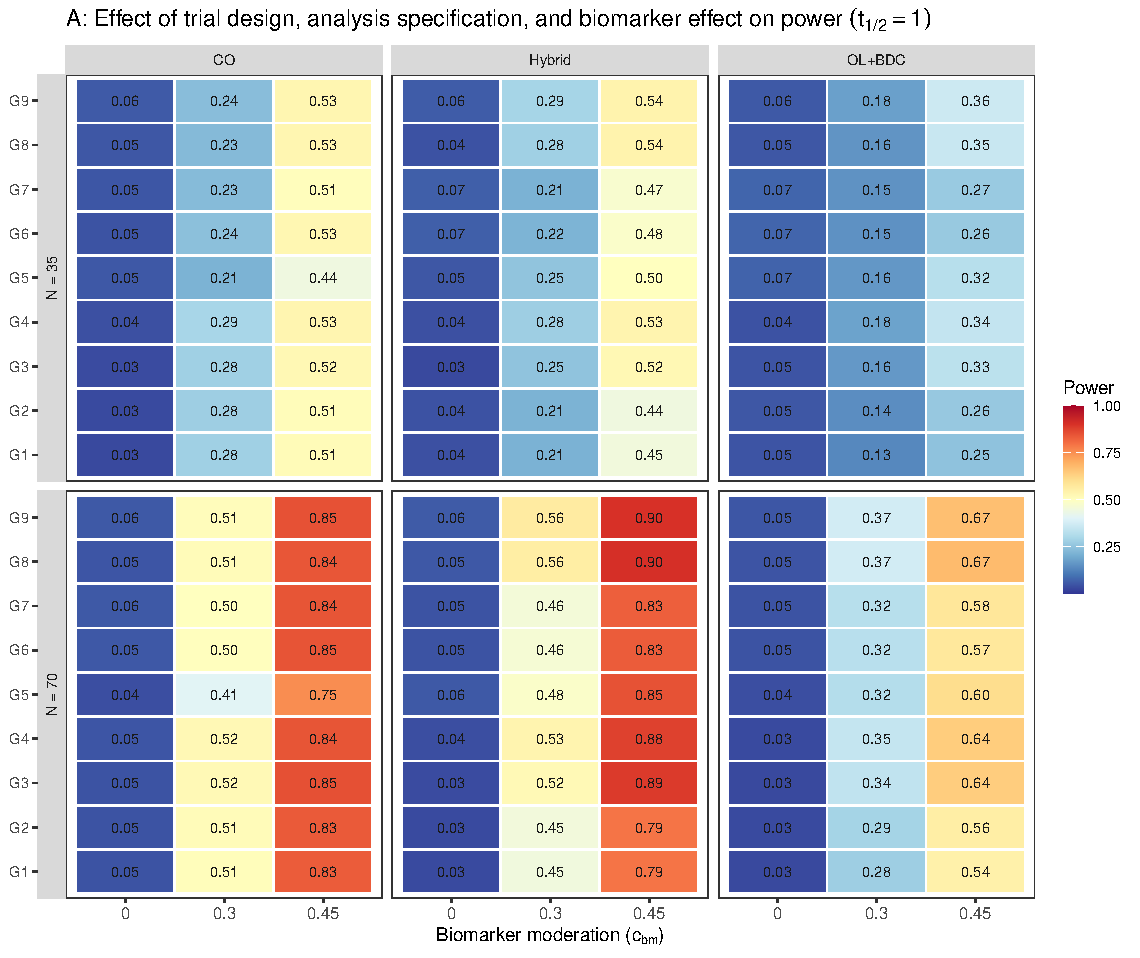
\includegraphics[width=0.95\linewidth]{../../figures/02xs-heatmap-hendrickson-a} \caption{Stage 3: power by trial design (columns), $N$ (row blocks) and analysis specification (rows within block) across $c_{bm} \in \{0, 0.30, 0.45\}$ at $t_{1/2} = 1.0$ weeks, exponential DGP, corrected simulation code ($n_{sim} = 500$). The $c_{bm} = 0$ column is Type I error.}\label{fig:fig-hendrickson-a}
\end{figure}

Figure \ref{fig:fig-hendrickson-b} varies the half-life at \(c_{bm} = 0.45\).

\begin{figure}
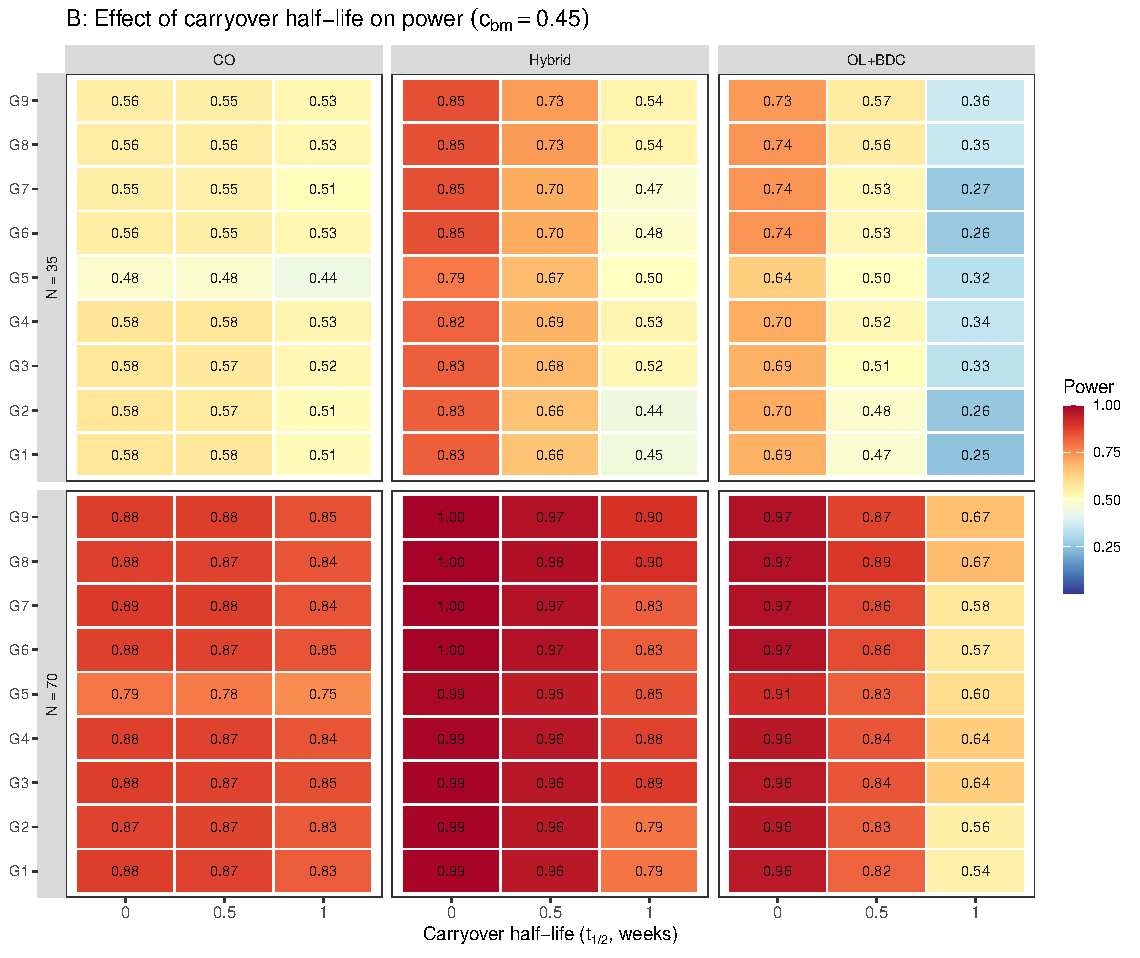
\includegraphics[width=0.95\linewidth]{../../figures/02xs-heatmap-hendrickson-b} \caption{Stage 3: power across $t_{1/2} \in \{0, 0.5, 1.0\}$ weeks at $c_{bm} = 0.45$, exponential DGP, corrected simulation code ($n_{sim} = 500$).}\label{fig:fig-hendrickson-b}
\end{figure}

\subsection*{Stage 4: external comparators on the same trials}\label{stage-4-external-comparators-on-the-same-trials}
\addcontentsline{toc}{subsection}{Stage 4: external comparators on the same trials}

Table \ref{tab:stage4-null} compares G9 with E0 and the expectancy-term family under the null. Under OL+BDC, E0 rejects at 0.100 and G9 at 0.060, and G9 stays at 0.048 to 0.052 on the prognostic rows.

\begin{table}
\centering
\caption{\label{tab:stage4-null}Stage 4: Type I error ($c_{bm} = 0$) at eight null
    scenarios on Hybrid ($N = 70$, $t_{1/2} = 0.5$ week unless
    stated; OL+BDC row is that design), $n_{sim} = 500$, same trial
    for every specification each replicate. The prognostic rows set
    one pathway parameter to 0.3; the prog-TV-grow row is a constant
    shift absorbed by the biomarker main effect and is identical to
    the Hybrid null row by construction. Two-MCSE band around 0.05:
    $[0.031, 0.069]$.}
\centering
\fontsize{9}{11}\selectfont
\begin{tabular}[t]{llllllllll}
\toprule
Cell & G1 & G3 & G4 & G6 & G8 & G9 & E0 & F1 & F1A0B\\
\midrule
Hybrid & 0.034 & 0.032 & 0.034 & 0.052 & 0.046 & 0.048 & 0.060 & 0.058 & 0.046\\
OL+BDC & 0.030 & 0.036 & 0.036 & 0.051 & 0.048 & 0.060 & 0.100 & 0.050 & 0.038\\
prog-BL 0.3 & 0.034 & 0.032 & 0.034 & 0.054 & 0.046 & 0.048 & 0.062 & 0.059 & 0.047\\
prog-TV-const 0.3 & 0.034 & 0.034 & 0.036 & 0.052 & 0.046 & 0.048 & 0.066 & 0.061 & 0.048\\
prog-TV-grow 0.3 & 0.034 & 0.032 & 0.034 & 0.052 & 0.046 & 0.048 & 0.060 & 0.058 & 0.046\\
\addlinespace
prog-PB 0.3 & 0.034 & 0.030 & 0.032 & 0.056 & 0.048 & 0.052 & 0.074 & 0.058 & 0.046\\
$t_{1/2} = 2$ wk & 0.034 & 0.038 & 0.042 & 0.052 & 0.054 & 0.062 & 0.066 & 0.059 & 0.047\\
Weibull $k = 2$ data & 0.032 & 0.032 & 0.032 & 0.052 & 0.046 & 0.052 & 0.060 & 0.058 & 0.058\\
\bottomrule
\end{tabular}
\end{table}

Table \ref{tab:stage4-alt} gives power. At \(t_{1/2} = 2\) weeks and \(c_{bm} = 0.25\), G9 reaches 0.281 against 0.192 for F1 and 0.228 for F1A0B.

\begin{table}
\centering
\caption{\label{tab:stage4-alt}Stage 4: power at five alternative scenarios (same
    specifications and $n_{sim}$ as the null table). G6 and G8 are
    the equal-size comparators for G9; E0 is liberal and its power
    is not comparable.}
\centering
\fontsize{9}{11}\selectfont
\begin{tabular}[t]{llllllllll}
\toprule
Cell & G1 & G3 & G4 & G6 & G8 & G9 & E0 & F1 & F1A0B\\
\midrule
Hybrid, $c_{bm} = 0.45$ & 0.934 & 0.950 & 0.950 & 0.962 & 0.972 & 0.968 & 0.932 & 0.952 & 0.950\\
Hybrid, $c_{bm} = 0.25$ & 0.510 & 0.542 & 0.544 & 0.564 & 0.574 & 0.584 & 0.546 & 0.538 & 0.500\\
OL+BDC, $c_{bm} = 0.45$ & 0.842 & 0.842 & 0.825 & 0.865 & 0.871 & 0.863 & 0.866 & 0.848 & 0.812\\
$t_{1/2} = 2$ wk, $c_{bm} = 0.25$ & 0.180 & 0.242 & 0.265 & 0.196 & 0.257 & 0.281 & 0.284 & 0.192 & 0.228\\
Weibull $k = 2$ data, $c_{bm} = 0.25$ & 0.630 & 0.610 & 0.631 & 0.653 & 0.655 & 0.661 & 0.612 & 0.652 & 0.614\\
\bottomrule
\end{tabular}
\end{table}

\subsubsection*{Scenario grids}\label{scenario-grids}
\addcontentsline{toc}{subsubsection}{Scenario grids}

Table \ref{tab:stage4-grid-null} crosses the scenarios with two sample sizes. The G9 Type I error is 0.034 to 0.067 in all fourteen cells.

\begin{table}
\centering
\caption{\label{tab:stage4-grid-null}Stage 4, scenario grids: Type I error ($c_{bm} = 0$) on
    Hybrid at $N \in \{35, 70\}$ under a Weibull decay analyzed as
    exponential, a true half-life below, at the boundary of and above
    G4's candidate grid, and two autocorrelations ($t_{1/2} = 0.5$ week and $\rho = 0.7$ unless
    stated; $n_{sim} = 500$; band $[0.031, 0.069]$).}
\centering
\fontsize{9}{11}\selectfont
\begin{tabular}[t]{lrlllllllll}
\toprule
Scenario & $N$ & G1 & G3 & G4 & G6 & G8 & G9 & E0 & F1 & F1A0B\\
\midrule
Weibull $k = 0.5$ data & 35 & 0.038 & 0.040 & 0.048 & 0.040 & 0.042 & 0.052 & 0.054 & 0.044 & 0.044\\
Weibull $k = 0.5$ data & 70 & 0.026 & 0.028 & 0.028 & 0.034 & 0.040 & 0.048 & 0.060 & 0.042 & 0.050\\
Weibull $k = 2$ data & 35 & 0.038 & 0.032 & 0.040 & 0.040 & 0.042 & 0.038 & 0.054 & 0.044 & 0.032\\
Weibull $k = 2$ data & 70 & 0.026 & 0.028 & 0.030 & 0.036 & 0.042 & 0.038 & 0.062 & 0.043 & 0.049\\
$t_{1/2} = 0.2$ wk & 35 & 0.038 & 0.040 & 0.040 & 0.040 & 0.038 & 0.038 & 0.054 & 0.044 & 0.030\\
\addlinespace
$t_{1/2} = 0.2$ wk & 70 & 0.026 & 0.026 & 0.028 & 0.036 & 0.032 & 0.034 & 0.060 & 0.044 & 0.047\\
$t_{1/2} = 2$ wk & 35 & 0.036 & 0.022 & 0.034 & 0.042 & 0.050 & 0.056 & 0.048 & 0.046 & 0.028\\
$t_{1/2} = 2$ wk & 70 & 0.026 & 0.030 & 0.034 & 0.034 & 0.046 & 0.058 & 0.056 & 0.042 & 0.056\\
$t_{1/2} = 4$ wk & 35 & 0.036 & 0.022 & 0.044 & 0.042 & 0.044 & 0.064 & 0.050 & 0.046 & 0.030\\
$t_{1/2} = 4$ wk & 70 & 0.026 & 0.026 & 0.038 & 0.036 & 0.042 & 0.067 & 0.060 & 0.042 & 0.046\\
\addlinespace
$\rho = 0.5$ & 35 & 0.032 & 0.036 & 0.040 & 0.044 & 0.046 & 0.060 & 0.056 & 0.048 & 0.052\\
$\rho = 0.5$ & 70 & 0.024 & 0.030 & 0.028 & 0.030 & 0.044 & 0.046 & 0.062 & 0.044 & 0.034\\
$\rho = 0.9$ & 35 & 0.016 & 0.018 & 0.016 & 0.038 & 0.036 & 0.034 & 0.040 & 0.034 & 0.030\\
$\rho = 0.9$ & 70 & 0.018 & 0.018 & 0.022 & 0.044 & 0.050 & 0.048 & 0.034 & 0.044 & 0.050\\
\bottomrule
\end{tabular}
\end{table}

Table \ref{tab:stage4-grid-alt} gives power. At \(\rho = 0.9\) and \(N = 35\), G9 reaches 0.808 against 0.684 for G1 and 0.608 for E0.

\begin{table}
\centering
\caption{\label{tab:stage4-grid-alt}Stage 4, scenario grids: power at one alternative per
    scenario (same cells and $n_{sim}$ as the null table; $c_{bm} =
    0.30$ for the autocorrelation rows because 0.45 is infeasible at
    $\rho = 0.9$).}
\centering
\fontsize{9}{11}\selectfont
\begin{tabular}[t]{lrlllllllll}
\toprule
Scenario & $N$ & G1 & G3 & G4 & G6 & G8 & G9 & E0 & F1 & F1A0B\\
\midrule
Weibull $k = 0.5$ data, $c_{bm} = 0.45$ & 35 & 0.538 & 0.552 & 0.572 & 0.548 & 0.586 & 0.588 & 0.586 & 0.541 & 0.523\\
Weibull $k = 0.5$ data, $c_{bm} = 0.45$ & 70 & 0.878 & 0.894 & 0.889 & 0.900 & 0.915 & 0.913 & 0.876 & 0.891 & 0.891\\
Weibull $k = 2$ data, $c_{bm} = 0.45$ & 35 & 0.830 & 0.814 & 0.828 & 0.850 & 0.848 & 0.850 & 0.794 & 0.826 & 0.809\\
Weibull $k = 2$ data, $c_{bm} = 0.45$ & 70 & 0.994 & 0.990 & 0.994 & 0.996 & 0.994 & 0.994 & 0.986 & 0.992 & 0.992\\
$t_{1/2} = 0.2$ wk, $c_{bm} = 0.25$ & 35 & 0.348 & 0.344 & 0.342 & 0.340 & 0.342 & 0.338 & 0.336 & 0.328 & 0.292\\
\addlinespace
$t_{1/2} = 0.2$ wk, $c_{bm} = 0.25$ & 70 & 0.632 & 0.626 & 0.628 & 0.659 & 0.659 & 0.657 & 0.614 & 0.645 & 0.659\\
$t_{1/2} = 2$ wk, $c_{bm} = 0.25$ & 35 & 0.108 & 0.124 & 0.150 & 0.112 & 0.146 & 0.168 & 0.160 & 0.114 & 0.134\\
$t_{1/2} = 2$ wk, $c_{bm} = 0.25$ & 70 & 0.176 & 0.220 & 0.235 & 0.185 & 0.233 & 0.254 & 0.246 & 0.177 & 0.218\\
$t_{1/2} = 4$ wk, $c_{bm} = 0.25$ & 35 & 0.058 & 0.066 & 0.080 & 0.064 & 0.080 & 0.102 & 0.098 & 0.066 & 0.084\\
$t_{1/2} = 4$ wk, $c_{bm} = 0.25$ & 70 & 0.084 & 0.104 & 0.137 & 0.092 & 0.134 & 0.139 & 0.140 & 0.087 & 0.105\\
\addlinespace
$\rho = 0.5$, $c_{bm} = 0.30$ & 35 & 0.280 & 0.300 & 0.310 & 0.284 & 0.288 & 0.306 & 0.358 & 0.264 & 0.248\\
$\rho = 0.5$, $c_{bm} = 0.30$ & 70 & 0.542 & 0.546 & 0.552 & 0.595 & 0.606 & 0.596 & 0.610 & 0.522 & 0.456\\
$\rho = 0.9$, $c_{bm} = 0.30$ & 35 & 0.684 & 0.734 & 0.717 & 0.785 & 0.808 & 0.808 & 0.608 & 0.794 & 0.772\\
$\rho = 0.9$, $c_{bm} = 0.30$ & 70 & 0.974 & 0.980 & 0.980 & 0.994 & 0.990 & 0.994 & 0.910 & 0.994 & 0.994\\
\bottomrule
\end{tabular}
\end{table}

\subsubsection*{Dropout}\label{dropout}
\addcontentsline{toc}{subsubsection}{Dropout}

Table \ref{tab:stage4-dropout} imposes monotone dropout. The G9 Type I error is 0.026 to 0.062, and at rate 0.3 and \(N = 35\) its power is 0.617 (MAR) and 0.649 (MCAR).

\begin{table}
\centering
\caption{\label{tab:stage4-dropout}Stage 4: Type I error and power under monotone dropout
    (Hybrid, $t_{1/2} = 0.5$ week; the rate is the fraction of
    patients with an incomplete series; $n_{sim} = 500$; band $[0.031,
    0.069]$).}
\centering
\fontsize{9}{11}\selectfont
\begin{tabular}[t]{lllllllll}
\toprule
\multicolumn{1}{c}{ } & \multicolumn{4}{c}{Type I error} & \multicolumn{4}{c}{Power, $c_{bm} = 0.45$} \\
\cmidrule(l{3pt}r{3pt}){2-5} \cmidrule(l{3pt}r{3pt}){6-9}
Dropout (rate, $N$) & G1 & G8 & G9 & F1 & G1 & G8 & G9 & F1\\
\midrule
MAR 0.1, $N = 35$ & 0.028 & 0.042 & 0.050 & 0.046 & 0.672 & 0.719 & 0.717 & 0.662\\
MAR 0.2, $N = 35$ & 0.034 & 0.046 & 0.052 & 0.048 & 0.638 & 0.687 & 0.687 & 0.607\\
MAR 0.3, $N = 35$ & 0.030 & 0.044 & 0.054 & 0.042 & 0.596 & 0.630 & 0.617 & 0.571\\
MCAR 0.1, $N = 35$ & 0.030 & 0.048 & 0.062 & 0.046 & 0.674 & 0.716 & 0.718 & 0.666\\
MCAR 0.2, $N = 35$ & 0.024 & 0.040 & 0.054 & 0.044 & 0.644 & 0.686 & 0.681 & 0.632\\
\addlinespace
MCAR 0.3, $N = 35$ & 0.024 & 0.036 & 0.042 & 0.038 & 0.608 & 0.646 & 0.649 & 0.584\\
MAR 0.1, $N = 70$ & 0.026 & 0.040 & 0.040 & 0.042 & 0.956 & 0.980 & 0.976 & 0.958\\
MAR 0.2, $N = 70$ & 0.022 & 0.038 & 0.042 & 0.040 & 0.936 & 0.972 & 0.976 & 0.932\\
MAR 0.3, $N = 70$ & 0.038 & 0.040 & 0.042 & 0.036 & 0.910 & 0.940 & 0.948 & 0.920\\
MCAR 0.1, $N = 70$ & 0.022 & 0.036 & 0.040 & 0.042 & 0.958 & 0.978 & 0.978 & 0.952\\
\addlinespace
MCAR 0.2, $N = 70$ & 0.020 & 0.032 & 0.026 & 0.026 & 0.950 & 0.976 & 0.970 & 0.956\\
MCAR 0.3, $N = 70$ & 0.024 & 0.032 & 0.040 & 0.030 & 0.926 & 0.956 & 0.952 & 0.924\\
\bottomrule
\end{tabular}
\end{table}

Table \ref{tab:stage3-coverage} gives interval coverage. G8 covers at 0.950 to 0.959 on average, and G9 at 0.934 to 0.947.

\begin{table}
\centering
\caption{\label{tab:stage3-coverage}Coverage of the nominal 95 percent CR2 interval for G8
      and G9 over the alternative cells of the supplementary study, on the
      calibrated scale ($\theta = -c_{bm}\sigma_{BR}$). The
      Satterthwaite degrees of freedom are not stored per replicate
      and were recovered from the stored $t$ and $p$ where $|t| \ge
      0.5$; the remaining replicates are classified as covering, not
      covering, or ambiguous, which gives the lower and upper bounds.
      From `34-referee-reanalysis.R`.}
\centering
\fontsize{9}{11}\selectfont
\begin{tabular}[t]{lrrll}
\toprule
Method & $N$ & Cells & Mean coverage (lower, upper) & Minimum (lower)\\
\midrule
G8 & 35 & 21 & 0.950, 0.959 & 0.938\\
G8 & 70 & 28 & 0.950, 0.954 & 0.915\\
G9 & 35 & 21 & 0.938, 0.947 & 0.890\\
G9 & 70 & 28 & 0.934, 0.940 & 0.873\\
\bottomrule
\end{tabular}
\end{table}

Table \ref{tab:heavy-missing} is the heavy-missingness case. The conventional \(\kappa\) of G9 is 0.46 and 0.49, and the robust \(\kappa\) is 0.78 and 0.86.

\begin{table}
\centering
\caption{\label{tab:heavy-missing}Heavy-missingness stress case (per-occasion MCAR 0.3,
      $N = 35$, 500 replicates): dispersion of the interaction
      estimates on the calibrated scale and the calibration ratio on
      the conventional scale ($\kappa$, mean SE over SD) and a robust
      one (median SE over 1.4826 times the median absolute
      deviation). From `34-referee-reanalysis.R`.}
\centering
\fontsize{9}{11}\selectfont
\begin{tabular}[t]{llllllll}
\toprule
Cell & Method & SD of estimates & MAD-based SD & Max $|\hat\beta|$ & $\kappa$ & Robust $\kappa$ & Rejection\\
\midrule
$c_{bm} = 0.45$ & G6 & 6.1 & 3.1 & 89 & 0.58 & 0.94 & 0.075\\
$c_{bm} = 0.45$ & G8 & 7.5 & 3.9 & 110 & 0.57 & 0.91 & 0.085\\
$c_{bm} = 0.45$ & G9 & 12.4 & 5.2 & 137 & 0.46 & 0.78 & 0.083\\
$c_{bm} = 0.45$ & F1 & 6.1 & 3.2 & 86 & 0.59 & 0.93 & 0.075\\
null & G6 & 6.1 & 3.3 & 82 & 0.61 & 0.90 & 0.020\\
null & G8 & 7.6 & 4.2 & 102 & 0.60 & 0.88 & 0.024\\
null & G9 & 12.4 & 5.1 & 131 & 0.49 & 0.86 & 0.022\\
null & F1 & 6.2 & 3.5 & 78 & 0.62 & 0.92 & 0.024\\
\bottomrule
\end{tabular}
\end{table}

\subsection*{Stage 5: prognostic confounds, feasibility, and random effects}\label{stage-5-prognostic-confounds-feasibility-and-random-effects}
\addcontentsline{toc}{subsection}{Stage 5: prognostic confounds, feasibility, and random effects}

\subsubsection*{Prognostic confounds at two strengths}\label{prognostic-confounds-at-two-strengths}
\addcontentsline{toc}{subsubsection}{Prognostic confounds at two strengths}

Table \ref{tab:stage5-size} gives size at strength 0.3. The G9 Type I error is 0.044 to 0.050 on the four pathways.

\begin{table}
\centering
\caption{\label{tab:stage5-size}Stage 5: Type I error of G9 and F1A0B under each
    prognostic pathway at confound strength 0.3, with no true
    interaction ($c_{bm} = 0$), Hybrid, $t_{1/2} = 0.5$ week,
    $n_{sim} = 500$ (band $[0.031, 0.069]$). The strength-0.6 cells
    on prog-BL, prog-PB and prog-TV-const were generated under a
    repaired covariance matrix, that is, a different DGP, and are
    not evidence about size (see text). The constant-shift row is
    identical to the no-confound null by construction.}
\centering
\fontsize{9}{11}\selectfont
\begin{tabular}[t]{lllll}
\toprule
\multicolumn{1}{c}{ } & \multicolumn{2}{c}{G9} & \multicolumn{2}{c}{F1A0B} \\
\cmidrule(l{3pt}r{3pt}){2-3} \cmidrule(l{3pt}r{3pt}){4-5}
Pathway & $N = 35$ & $N = 70$ & $N = 35$ & $N = 70$\\
\midrule
prog-BL & 0.048 & 0.044 & 0.044 & 0.034\\
prog-TV-const & 0.050 & 0.048 & 0.046 & 0.034\\
prog-TV-shift (constant) & 0.046 & 0.046 & 0.046 & 0.034\\
prog-PB & 0.046 & 0.044 & 0.046 & 0.034\\
\bottomrule
\end{tabular}
\end{table}

Table \ref{tab:stage5-power} gives power at two strengths. At strength 0.3 and \(N = 35\) the G9 power is 0.778 to 0.798, against a no-confound reference of 0.759, and the strength-0.6 cells are an artifact.

\begin{table}
\centering
\caption{\label{tab:stage5-power}Stage 5: power of G9 and F1A0B with a true
    interaction ($c_{bm} = 0.45$) and a co-occurring prognostic
    confound, same layout as the size table. The no-confound
    reference for G9 is 0.759 at $N = 35$ and 0.969 at $N = 70$
    (1{,}000 replicates, a different job from these cells, so the
    comparison is unpaired). Strength-0.6 cells on prog-BL, prog-PB
    and prog-TV-const are a data-generating artifact, not a confound
    effect (see text).}
\centering
\fontsize{9}{11}\selectfont
\begin{tabular}[t]{lllllllll}
\toprule
\multicolumn{1}{c}{ } & \multicolumn{2}{c}{G9, $N = 35$} & \multicolumn{2}{c}{G9, $N = 70$} & \multicolumn{2}{c}{F1A0B, $N = 35$} & \multicolumn{2}{c}{F1A0B, $N = 70$} \\
\cmidrule(l{3pt}r{3pt}){2-3} \cmidrule(l{3pt}r{3pt}){4-5} \cmidrule(l{3pt}r{3pt}){6-7} \cmidrule(l{3pt}r{3pt}){8-9}
Pathway & 0.3 & 0.6 & 0.3 & 0.6 & 0.3 & 0.6 & 0.3 & 0.6\\
\midrule
prog-BL & 0.782 & 0.758 & 0.976 & 0.960 & 0.738 & 0.702 & 0.950 & 0.920\\
prog-TV-const & 0.782 & 0.730 & 0.968 & 0.950 & 0.502 & 0.482 & 0.772 & 0.702\\
prog-TV-shift (constant) & 0.778 & 0.756 & 0.970 & 0.966 & 0.778 & 0.756 & 0.970 & 0.966\\
prog-PB & 0.798 & 0.741 & 0.968 & 0.940 & 0.597 & 0.562 & 0.853 & 0.794\\
\bottomrule
\end{tabular}
\end{table}

\subsubsection*{The strength-0.6 loss is a data-generating artifact}\label{the-strength-0.6-loss-is-a-data-generating-artifact}
\addcontentsline{toc}{subsubsection}{The strength-0.6 loss is a data-generating artifact}

Table \ref{tab:stage5-pd} shows that every strength-0.6 cell with the interaction had a matrix that was not positive definite on all four paths. The repair moved the contrast from \(-3.53\) to \(-2.38\) for prog-PB and from \(-3.26\) to \(-1.81\) for prog-TV-const.

\begin{table}
\centering
\caption{\label{tab:stage5-pd}Stage 5: positive definiteness of the raw joint
    covariance matrix on the four Hybrid paths, and the population
    on-drug minus off-drug slope contrast of the outcome on the
    biomarker before and after the silent repair, for the prognostic
    cells at $c_{bm} = 0.45$ and the strength-0.6 null cells
    (computed from the matrix, no simulation). The contrast is the
    population value of the interaction term.}
\centering
\fontsize{9}{11}\selectfont
\begin{tabular}[t]{lrrrlll}
\toprule
Pathway & Strength & $c_{bm}$ & Paths repaired & Min. eigenvalue & Contrast, raw & Contrast, repaired\\
\midrule
none & 0.0 & 0.45 & 0 & 0.180 & -3.26 & -3.26\\
prog-BL & 0.3 & 0.45 & 0 & 0.145 & -3.26 & -3.26\\
prog-BL & 0.6 & 0.00 & 0 & 0.184 & 0.00 & 0.00\\
prog-BL & 0.6 & 0.45 & 4 & -0.110 & -3.26 & -3.00\\
prog-PB & 0.3 & 0.45 & 0 & 0.010 & -3.40 & -3.40\\
\addlinespace
prog-PB & 0.6 & 0.00 & 4 & -0.240 & -0.27 & -0.23\\
prog-PB & 0.6 & 0.45 & 4 & -0.642 & -3.53 & -2.38\\
prog-TV-const & 0.3 & 0.45 & 0 & 0.011 & -3.26 & -3.26\\
prog-TV-const & 0.6 & 0.00 & 4 & -0.354 & 0.00 & 0.00\\
prog-TV-const & 0.6 & 0.45 & 4 & -0.853 & -3.26 & -1.81\\
\bottomrule
\end{tabular}
\end{table}

\subsubsection*{The feasibility bound for a prognostic correlation}\label{the-feasibility-bound-for-a-prognostic-correlation}
\addcontentsline{toc}{subsubsection}{The feasibility bound for a prognostic correlation}

Table \ref{tab:stage5-ceiling} gives the closed-form bounds. The bound for \(c_{pb}\) falls from 0.513 alone to 0.451 given \(c_{bm} = 0.3\), so strength 0.6 is infeasible.

\begin{table}
\centering
\caption{\label{tab:stage5-ceiling}Stage 5: exact feasibility bounds (the `Ceiling` column)
    for each biomarker correlation (the `Coupling` column), alone and
    given a fixed biomarker-response correlation $c_{bm}$, Hybrid
    design (minimum over paths), $t_{1/2} = 0.5$ week, $\rho = 0.7$,
    $c_1 = 0.2$. Each bound is verified by the smallest eigenvalue
    of the full correlation matrix being positive at $0.999$ times
    and negative at $1.001$ times the stated value.}
\centering
\fontsize{9}{11}\selectfont
\begin{tabular}[t]{lll}
\toprule
Coupling & Given & Ceiling\\
\midrule
$c_{bm}$ & alone & 0.518\\
$c_{pb}$ & alone & 0.513\\
$c_{tv}$ & alone & 0.513\\
$c_{bl}$ & alone & 1.000\\
$c_{pb}$ & $c_{bm}$ = 0.3 & 0.451\\
\addlinespace
$c_{tv}$ & $c_{bm}$ = 0.3 & 0.451\\
$c_{bl}$ & $c_{bm}$ = 0.3 & 0.815\\
$c_{pb}$ & $c_{bm}$ = 0.45 & 0.306\\
$c_{tv}$ & $c_{bm}$ = 0.45 & 0.306\\
$c_{bl}$ & $c_{bm}$ = 0.45 & 0.496\\
\bottomrule
\end{tabular}
\end{table}

\subsubsection*{Robustness up to the feasibility bound}\label{robustness-up-to-the-feasibility-bound}
\addcontentsline{toc}{subsubsection}{Robustness up to the feasibility bound}

Table \ref{tab:stage5-ladder} runs confounds inside the bounds. The G9 Type I error is 0.042 to 0.046, and its power at \(c_{bm} = 0.30\) is 0.682 to 0.780.

\begin{table}
\centering
\caption{\label{tab:stage5-ladder}Stage 5: rejection rate on the feasible
    prognostic-confound ladder (Hybrid, $N = 70$, $t_{1/2} = 0.5$
    week, $n_{sim} = 500$). Rows with $c_{bm} = 0$ are Type I error
    (band $[0.031, 0.069]$); the others are power. Every cell passed
    the pre-flight positive-definiteness check.}
\centering
\fontsize{9}{11}\selectfont
\begin{tabular}[t]{llllllllll}
\toprule
Cell & G1 & G3 & G4 & G6 & G8 & G9 & E0 & F1 & F1A0B\\
\midrule
prog-PB 0.40, $c_{bm} = 0.00$ & 0.030 & 0.028 & 0.028 & 0.040 & 0.042 & 0.044 & 0.064 & 0.043 & 0.059\\
prog-PB 0.40, $c_{bm} = 0.30$ & 0.706 & 0.714 & 0.721 & 0.737 & 0.752 & 0.757 & 0.750 & 0.680 & 0.713\\
prog-PB 0.45, $c_{bm} = 0.00$ & 0.028 & 0.030 & 0.030 & 0.040 & 0.040 & 0.044 & 0.062 & 0.040 & 0.048\\
prog-PB 0.45, $c_{bm} = 0.30$ & 0.694 & 0.730 & 0.729 & 0.751 & 0.776 & 0.780 & 0.756 & 0.694 & 0.712\\
prog-TV-const 0.40, $c_{bm} = 0.00$ & 0.024 & 0.028 & 0.022 & 0.040 & 0.038 & 0.046 & 0.060 & 0.046 & 0.046\\
\addlinespace
prog-TV-const 0.40, $c_{bm} = 0.30$ & 0.678 & 0.680 & 0.687 & 0.692 & 0.734 & 0.729 & 0.694 & 0.671 & 0.695\\
prog-TV-const 0.45, $c_{bm} = 0.00$ & 0.028 & 0.028 & 0.026 & 0.038 & 0.038 & 0.044 & 0.058 & 0.046 & 0.045\\
prog-TV-const 0.45, $c_{bm} = 0.30$ & 0.662 & 0.680 & 0.684 & 0.704 & 0.720 & 0.721 & 0.706 & 0.679 & 0.685\\
prog-BL 0.45, $c_{bm} = 0.00$ & 0.026 & 0.028 & 0.026 & 0.032 & 0.042 & 0.046 & 0.058 & 0.047 & 0.059\\
prog-BL 0.45, $c_{bm} = 0.45$ & 0.958 & 0.970 & 0.970 & 0.976 & 0.976 & 0.978 & 0.958 & 0.968 & 0.972\\
\addlinespace
prog-BL 0.60, $c_{bm} = 0.00$ & 0.030 & 0.032 & 0.030 & 0.030 & 0.040 & 0.043 & 0.058 & 0.045 & 0.059\\
prog-BL 0.60, $c_{bm} = 0.30$ & 0.656 & 0.660 & 0.665 & 0.681 & 0.708 & 0.694 & 0.684 & 0.648 & 0.675\\
prog-BL 0.80, $c_{bm} = 0.00$ & 0.026 & 0.030 & 0.028 & 0.034 & 0.042 & 0.042 & 0.060 & 0.046 & 0.050\\
prog-BL 0.80, $c_{bm} = 0.30$ & 0.638 & 0.666 & 0.664 & 0.679 & 0.688 & 0.682 & 0.692 & 0.650 & 0.660\\
\bottomrule
\end{tabular}
\end{table}

Table \ref{tab:stage5-largen} tests larger samples under prog-PB. At \(c_{pb} = 0.45\) the G9 rejection rate rises from 0.044 at \(N = 70\) to 0.059 at 140 and 0.062 at 280, and F1 is at 0.067.

\begin{table}
\centering
\caption{\label{tab:stage5-largen}Stage 5: Type I error under prog-PB with no true
    interaction at larger samples (Hybrid, $t_{1/2} = 0.5$ week;
    $n_{sim} = 1{,}000$ at $N = 140$ and $280$, band $[0.036,
    0.064]$; the $N = 70$ row is from the ladder, $n_{sim} = 500$).}
\centering
\fontsize{9}{11}\selectfont
\begin{tabular}[t]{llllllllll}
\toprule
Cell & G1 & G3 & G4 & G6 & G8 & G9 & E0 & F1 & F1A0B\\
\midrule
$c_{pb} = 0.30$, $N = 140$ & 0.044 & 0.043 & 0.043 & 0.058 & 0.055 & 0.055 & 0.068 & 0.057 & 0.049\\
$c_{pb} = 0.30$, $N = 280$ & 0.053 & 0.045 & 0.052 & 0.065 & 0.063 & 0.063 & 0.071 & 0.067 & 0.060\\
$c_{pb} = 0.45$, $N = 70$ & 0.028 & 0.030 & 0.030 & 0.040 & 0.040 & 0.044 & 0.062 & 0.040 & 0.048\\
$c_{pb} = 0.45$, $N = 140$ & 0.046 & 0.042 & 0.045 & 0.059 & 0.056 & 0.059 & 0.072 & 0.057 & 0.046\\
$c_{pb} = 0.45$, $N = 280$ & 0.055 & 0.049 & 0.054 & 0.066 & 0.062 & 0.062 & 0.077 & 0.067 & 0.061\\
\bottomrule
\end{tabular}
\end{table}

\subsubsection*{A biomarker that predicts the rate of natural-history change}\label{a-biomarker-that-predicts-the-rate-of-natural-history-change}
\addcontentsline{toc}{subsubsection}{A biomarker that predicts the rate of natural-history change}

Table \ref{tab:stage5-trend} shows the pathway that the feasibility bound does not limit. Under the null, G8 rejects at 0.068, G9 at 0.074 and F1 at 0.059.

\begin{table}
\centering
\caption{\label{tab:stage5-trend}Stage 5, referee-variant runs: rejection rate (MCSE),
      mean interaction estimate on the calibrated scale and
      calibration ratio under a biomarker that predicts the rate of
      natural-history change (coefficient 0.3), Hybrid, $N = 70$,
      $t_{1/2} = 0.5$ week, 1{,}000 replicates (two-MCSE band at the
      null $[0.036, 0.064]$). The true value at the alternative is
      $-3.6$.}
\centering
\fontsize{9}{11}\selectfont
\begin{tabular}[t]{lllll}
\toprule
Cell & Method & Rejection & Mean estimate & $\kappa$\\
\midrule
null ($c_{bm} = 0$) & G8 & 0.068 (0.008) & +0.21 & 0.96\\
 & G9 & 0.074 (0.008) & +0.19 & 0.94\\
 & F1 & 0.059 (0.008) & +0.11 & 0.98\\
$c_{bm} = 0.45$ & G8 & 0.954 (0.007) & -3.42 & 0.96\\
 & G9 & 0.954 (0.007) & -3.25 & 0.90\\
 & F1 & 0.938 (0.008) & -3.00 & 0.97\\
\bottomrule
\end{tabular}
\end{table}

Table \ref{tab:stage5-slope} adds a patient-specific linear trend. G9 rejects at 0.043 under the null and 0.969 at \(c_{bm} = 0.45\).

\begin{table}
\centering
\caption{\label{tab:stage5-slope}Stage 5, referee-variant runs: rejection rate (MCSE),
      mean interaction estimate and calibration ratio under a
      patient-specific linear trend in the natural-history component
      (SD 0.3 outcome units per week), Hybrid, $N = 70$,
      $t_{1/2} = 0.5$ week, 1{,}000 replicates.}
\centering
\fontsize{9}{11}\selectfont
\begin{tabular}[t]{lllll}
\toprule
Cell & Method & Rejection & Mean estimate & $\kappa$\\
\midrule
null ($c_{bm} = 0$) & G8 & 0.042 (0.006) & -0.02 & 1.01\\
 & G9 & 0.043 (0.006) & -0.01 & 0.99\\
 & F1 & 0.040 (0.006) & -0.02 & 1.01\\
$c_{bm} = 0.45$ & G8 & 0.970 (0.005) & -3.63 & 0.98\\
 & G9 & 0.969 (0.005) & -3.45 & 0.92\\
 & F1 & 0.955 (0.007) & -3.14 & 0.99\\
\bottomrule
\end{tabular}
\end{table}

Table \ref{tab:stage5-re} adds random slopes to G9. The variants differ from G9 by 0.010 or less.

\begin{table}
\centering
\caption{\label{tab:stage5-re}Stage 5: rejection rate of G9 and its three
    random-effects variants on twelve cells (Hybrid, $t_{1/2} = 0.5$
    week, $n_{sim} = 1{,}000$; $c_{bm} = 0$ rows are Type I error).
    The strength-0.6 rows were generated under the repaired matrix
    described above and are not evidence about the confound.}
\centering
\fontsize{9}{11}\selectfont
\begin{tabular}[t]{lllll}
\toprule
Cell & G9 & + slope on $t$ & + slope on $D_e$ & + both\\
\midrule
none, $c_{bm} = 0.00$, $N = 35$ & 0.050 & 0.050 & 0.050 & 0.046\\
none, $c_{bm} = 0.00$, $N = 70$ & 0.043 & 0.044 & 0.043 & 0.041\\
none, $c_{bm} = 0.45$, $N = 35$ & 0.759 & 0.762 & 0.766 & 0.769\\
none, $c_{bm} = 0.45$, $N = 70$ & 0.969 & 0.970 & 0.969 & 0.970\\
prog-PB 0.6, $c_{bm} = 0.00$, $N = 35$ & 0.060 & 0.060 & 0.059 & 0.060\\
\addlinespace
prog-PB 0.6, $c_{bm} = 0.00$, $N = 70$ & 0.047 & 0.046 & 0.047 & 0.047\\
prog-PB 0.6, $c_{bm} = 0.45$, $N = 35$ & 0.594 & 0.593 & 0.593 & 0.596\\
prog-PB 0.6, $c_{bm} = 0.45$, $N = 70$ & 0.860 & 0.859 & 0.858 & 0.858\\
prog-TV-const 0.6, $c_{bm} = 0.00$, $N = 35$ & 0.050 & 0.053 & 0.051 & 0.054\\
prog-TV-const 0.6, $c_{bm} = 0.00$, $N = 70$ & 0.044 & 0.044 & 0.043 & 0.040\\
\addlinespace
prog-TV-const 0.6, $c_{bm} = 0.45$, $N = 35$ & 0.489 & 0.488 & 0.489 & 0.485\\
prog-TV-const 0.6, $c_{bm} = 0.45$, $N = 70$ & 0.772 & 0.772 & 0.773 & 0.768\\
\bottomrule
\end{tabular}
\end{table}

\section*{Recommendation}\label{recommendation}
\addcontentsline{toc}{section}{Recommendation}

For a Hybrid trial we recommend G9, the exposure-weighted predictor with an AIC-selected half-life, refitted by REML and tested with CR2. Its size is about 0.055 at \(N \le 70\), so the selection step costs about half a point of size. A fixed 1-week analysis half-life with CR2 holds nominal size for at most two points of power. The recommendation is conditional on the extended DGP and the parameters simulated. A biomarker that predicts the natural-history trend biases every analysis examined.

\end{document}
